\section{Text Classification in Legal Judgments}\label{sec:text_classification}

% Explain the overall idea of the experiments

% How did we get to this setup?

% É possível usar TM techniques para classificar corretamente as sentenças?

This section presents the results for the classification experiments involving \gls{JEC}'s legal judgments. The section starts from the clarification of the experiments' purpose, that is, how they help on answering the research question. Then, it presents the details on the datasets used for the experiments, the pipelines of the experiments for Classical \gls{ML} and \gls{DL}, and the results and discussion.

\subsection{Experiment's Purpose}

% \begin{itemize}[noitemsep]
%     \item Primeiro experimento
%     \item Sentir dificuldades
%     \item Tornar compreensível a pipeline para o especialista
%     \item orange 3 - técnicas classicas
%     \item Como ele ajuda a responder  à segunda parte pergunta?
% \end{itemize}


The experiments' purpose is to answer the second part of the research question, that is, whether \gls{DL} techniques  can achieve better performance on \gls{JEC}'s cases classification when compared to Classical \gls{ML} techniques.
% Detail here.
Through the application of Classical and \gls{DL} techniques to the prediction of the \gls{JEC} legal judgments, we try to estimate the techniques' performance. 
Based on the results, we compare the techniques on how well they perform.

Besides the techniques comparison, in this section we tested the performance of the models using two datasets: legal judgments with full text and the legal judgments without the results section. Using  such strategy, one can notice whether including or not the results part, containing textual description of the label, impact in the models performance. 


In the experiments with Classical \gls{ML} techniques, we applied the open-source software Orange Data Mining (Version 3.22)~\cite{Demsar13}. Such tool aims at offering a variety of \gls{ML} and \gls{TM} techniques to the user in a simple way, without the need of any programming language. On the other hand, the experiments with \gls{DL} techniques (not available in Orange) required the use of several tools: the Python programming language, version 3.8; the Keras framework,Version 2.4.3~\cite{Chollet2015}; the Natural Language Toolkit (NLTK), version 3.5 ~\cite{Loper02} and the Scikit-Learn framework, version 0.24.1~\cite{Pedregosa2012}.\footnote{Pipeline for Orange3 and code for Keras are available at \url{https://github.com/thiagordp/text_classification_in_legal_docs}.}


Finally, the results presented in this section relate to the first contact of the researcher with the areas of study. Thus, considering the extensive amount of publications on legal text classification (detailed in Appendix~\ref{ap:rsl_ml_law}) and the researcher's expertise, the classification experiments produced small contributions, that is, the applications of Classical \gls{ML} and \gls{DL} techniques to the prediction of the results of legal judgments from \gls{JEC}.


\subsection{Datasets}

For the classification experiments, two datasets were used. Both are similar as before (JEC/UFSC legal judgments), but smaller because it was the first experiment performed. The judgments were issued between  January 2014 to May 2019.

The difference in the legal judgments from the two datasets used resides in their distinct textual structure.  In one of them, we removed the result's part, while in the other dataset,  we kept such part. Thus, considering the structure of a legal judgment described in Section~\ref{sec:embedding_dataset}, the first dataset contains legal judgments composed of two parts and less amount of text. The second dataset has three parts and more text.

Table~\ref{tab:cap4_class_distr_label} describes the quantity of examples for each label. 

\begin{table}[htb]
\centering
\caption{Label's distributions for text classification}
\label{tab:cap4_class_distr_label}
\footnotesize
\begin{tabular}{@{}lc@{}}
\toprule
\multicolumn{1}{c}{\textbf{Label}} & \textbf{Examples} \\ \midrule
Well Founded                            & 214               \\
Partly Founded                     & 379               \\
Dismissed without prejudice        & 10                \\
Not founded                        & 70                \\ \midrule
\multicolumn{1}{r}{\textbf{TOTAL}} & 673               \\ \bottomrule
\end{tabular}
\end{table}


In terms of quantitative information from the datasets, Table~\ref{tab:info_dataset_classification} presents the average count of tokens per document and the vocabulary size after each of the preprocessing steps for each dataset. As we will describe later, distinct preprocessing steps carried out for the experiments with Classical \gls{ML} and \gls{DL}. The information of tokens per document in the experiment with Classical ML was not available due to the restrictions from Orange Data Mining.


\begin{table}[htb]
\centering
\caption{Information on the datasets for classification}
\label{tab:info_dataset_classification}
\footnotesize
\begin{tabular}{@{}crrrr@{}}
\toprule
\textbf{\begin{tabular}[c]{@{}c@{}}Experiment's\\ Preprocessing\end{tabular}} & \multicolumn{1}{c}{\textbf{\begin{tabular}[c]{@{}c@{}}Tokens per \\ document\\ (w/ result)\end{tabular}}} & \multicolumn{1}{c}{\textbf{\begin{tabular}[c]{@{}c@{}}Vocabulary Size\\ (w/ result)\end{tabular}}} & \multicolumn{1}{c}{\textbf{\begin{tabular}[c]{@{}c@{}}Tokens per \\ document\\ (w/o result)\end{tabular}}} & \multicolumn{1}{c}{\textbf{\begin{tabular}[c]{@{}c@{}}Vocabulary Size\\ (w/o result)\end{tabular}}} \\ \midrule
\textbf{Classical ML}                                                         & -                                                                                                         & 12,994                                                                                                 & -                                                                                                          & 12,898                                                                                                   \\
\textbf{DL}                                                                   & 673.0                                                                                                         & 15,377                                                                                                  & 644.2                                                                                                          & 15,224                                                                                                   \\ \bottomrule
\end{tabular}
\end{table}

Similar to Section~\ref{sec:text_representation}, some of the legal judgments from the datasets presented more than one result, that is, they had more than one distinct labels. An example of this type of judgments happens when two people file a joint lawsuit against an airline, and the judge set distinct judgments for each of them. In those cases, the documents were replicated for each of the labels indicated on its results section, culminating in a total of 673 legal judgments, in each dataset, to serve as input for the experiments. Considering distinct legal judgments only, the dataset contains 665 documents.



% Cases' result = label in this work

\subsection{Pipelines}

This section describes the pipelines and experimental setup for the experiments with Classical \gls{ML} and \gls{DL} techniques.

The first set of classification experiments focused on the application of Classical \gls{ML} techniques. In such experiments, Orange 3 served as execution environment and followed the pipeline from Figure~\ref{fig:cap4_pipeline_superv_ml}. It receives two types of input: the texts from legal judgments, in a plain text format, and their labels, that is, the judgments' results. As outputs, the pipeline makes available the trained models and the test set which are passed to the prediction and evaluation step.


\begin{figure}[htb]
    \centering
    \caption{Pipeline for legal text classification using Classical ML techniques}
    \label{fig:cap4_pipeline_superv_ml}
    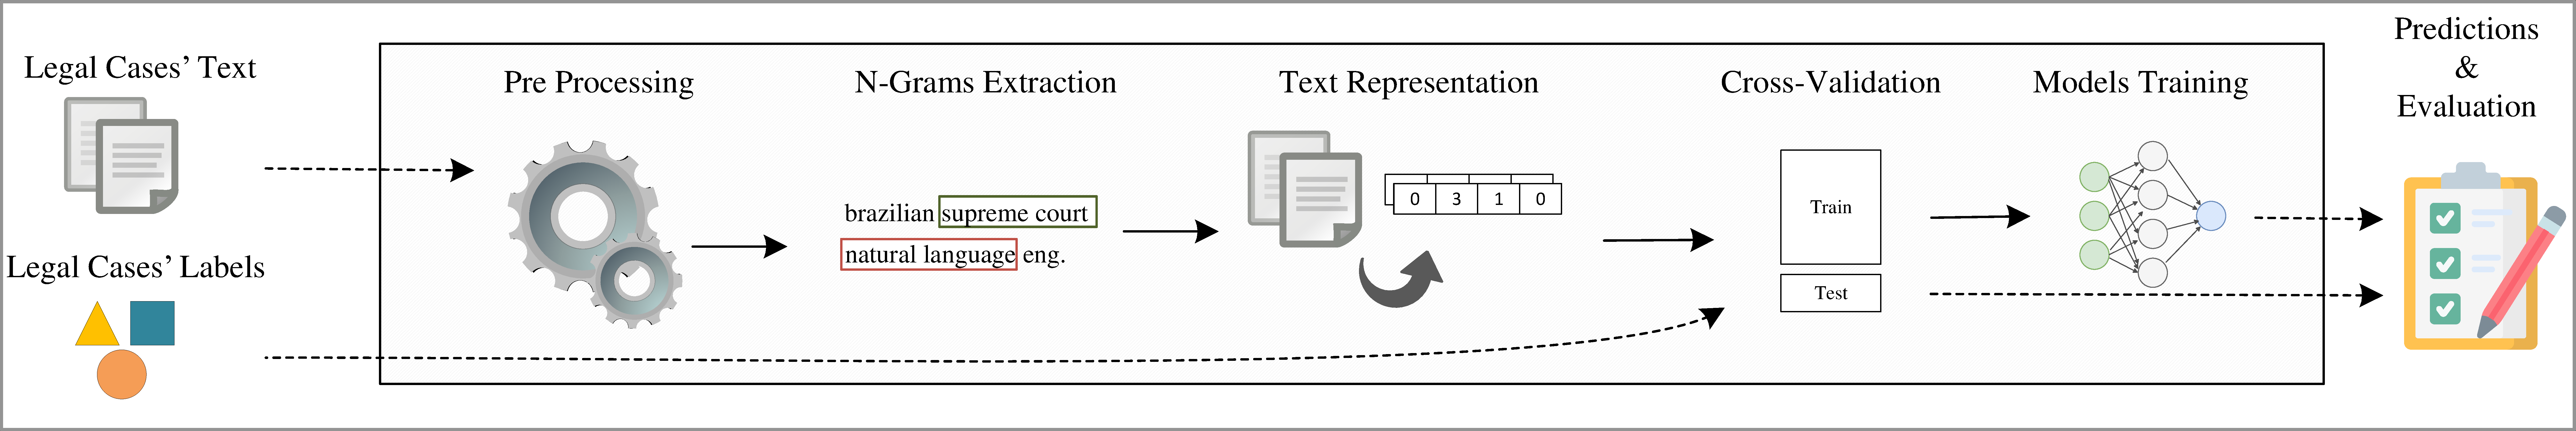
\includegraphics[width=\textwidth]{images/chapters/cap4_classification_pipeline.pdf}
\end{figure}


The first step in the pipeline is the data preprocessing. Considering the available techniques for preprocessing textual data, described in Chapter 2 and in the literature, in Appendix~\ref{ap:rsl_ml_law},  we applied transformation, tokenization, stemming and filtering, previously discussed in Section \ref{sec:bow}:

\begin{itemize}[noitemsep]
    \item \textbf{Tranformation:} the conversion to lower case to standardize the spelling of words.
    \item \textbf{Tokenization:} the application of regular expression ($\setminus w+$) to detect the pieces of texts, while removing spaces, symbols, and punctuation.
    \item \textbf{Stemming:} To reduce the variability of similar words, we applied Porter Stemmer~\cite{Porter1980}, a simple and efficient stemming algorithm to the Portuguese language. However, it may make errors, such as contracting the word \textit{morais} to \textit{morai}, instead of \textit{moral} (Portuguese words for singular and plural of \textit{moral}, respectively).
    \item \textbf{Filtering:} Removing stopwords, such as prepositions and articles to keep only the meaningful words.
\end{itemize}


The next step in the pipeline relates to the extraction of N-Grams, which detects sequences of two or more words that appear together consistently in the text. In this research, the limit of the length of N-grams was two. Bigger numbers of N-grams would lead to large textual representations.



After N-Grams Extraction, the numerical representations of the documents are created using the algorithm \gls{BOW}. In the experiments with Classical \gls{ML}, we used the \gls{TF} to calculate the values of the BOW model. 


The next step consists on dividing the dataset in two subsets: train and test sets. As described in Chapter~\ref{cap:ml_text}, there is the cross validation. In this research, $k$ was set to 10, that is, 90\% of the dataset used for training and 10\% for testing the models. Such proportion is a common choice to avoid bias while keeping some level of variance in the division of the folds~\cite{Airola2011}

The next step consists on training the models to predict the result of the judgments from \gls{JEC} according to the possible outcomes, as described in Section~\ref{sec:text_representation}. 
Experiments involved the following techniques: \gls{kNN}, \gls{SVM}, \gls{RF}, \gls{NN}, \gls{NB} and \gls{LR}. Table~\ref{tab:hyperparam_classification} presents the hyper-parameters applied to each technique, based on the values suggested by Orange 3.


% Incluir Tabela para descrever os parâmetros dos modelos.
\begin{table}[htb]
\centering
\caption{Hyperparameters for classification techniques}
\label{tab:hyperparam_classification}
\footnotesize
\begin{tabular}{cl}
\toprule
\textbf{Technique} & \multicolumn{1}{c}{\textbf{Hyper-parameters}} \\ \midrule

\gls{kNN} & \begin{tabular}[c]{@{}l@{}}Number of Neighbors: 4;\\ Distance Metric: Euclidean;\\ Weight: Uniform\end{tabular} \\ \hdashline

\gls{LR} & \begin{tabular}[c]{@{}l@{}}Regularization type: Ridge (L2);\\ C (strength): 1\end{tabular} \\\hdashline

\gls{NB} & -- \\ \hdashline

\gls{NN} & \begin{tabular}[c]{@{}l@{}}Hidden Layers: 2\\ Neurons in each layer: 100, 50;\\ Activation Function: tanh;\\ Solver: Stochastic Gradient descent (SGD)\end{tabular} \\ \hdashline

\gls{RF} & \begin{tabular}[c]{@{}l@{}}Number of Trees: 10;\\ Minimum subset size: 5\end{tabular} \\ \hdashline

\gls{SVM} & \begin{tabular}[c]{@{}l@{}}C (cost): 1.0;\\ $\epsilon$ (Regression loss): 0.1;\\ Kernel: \gls{RBF};\\ Iteration Limit: 100\end{tabular} \\ \bottomrule

\end{tabular}
\end{table}


Finally, there is the evaluation step, which estimates how well the models performed on predicting unseen legal judgments. To measure the performance, we used the Accuracy, detailed in Chapter~\ref{cap:ml_text}. At the time these experiments were published, only the accuracy was used.

The second set of experiments related to the application of \gls{DL} techniques to the prediction of the legal judgments' results. The pipeline used for these experiments is presented in Figure~\ref{fig:pipeline_dl}.

\begin{figure}[htb]
    \centering
    \caption{Pipeline for legal text classification using DL techniques}
    \label{fig:pipeline_dl}
    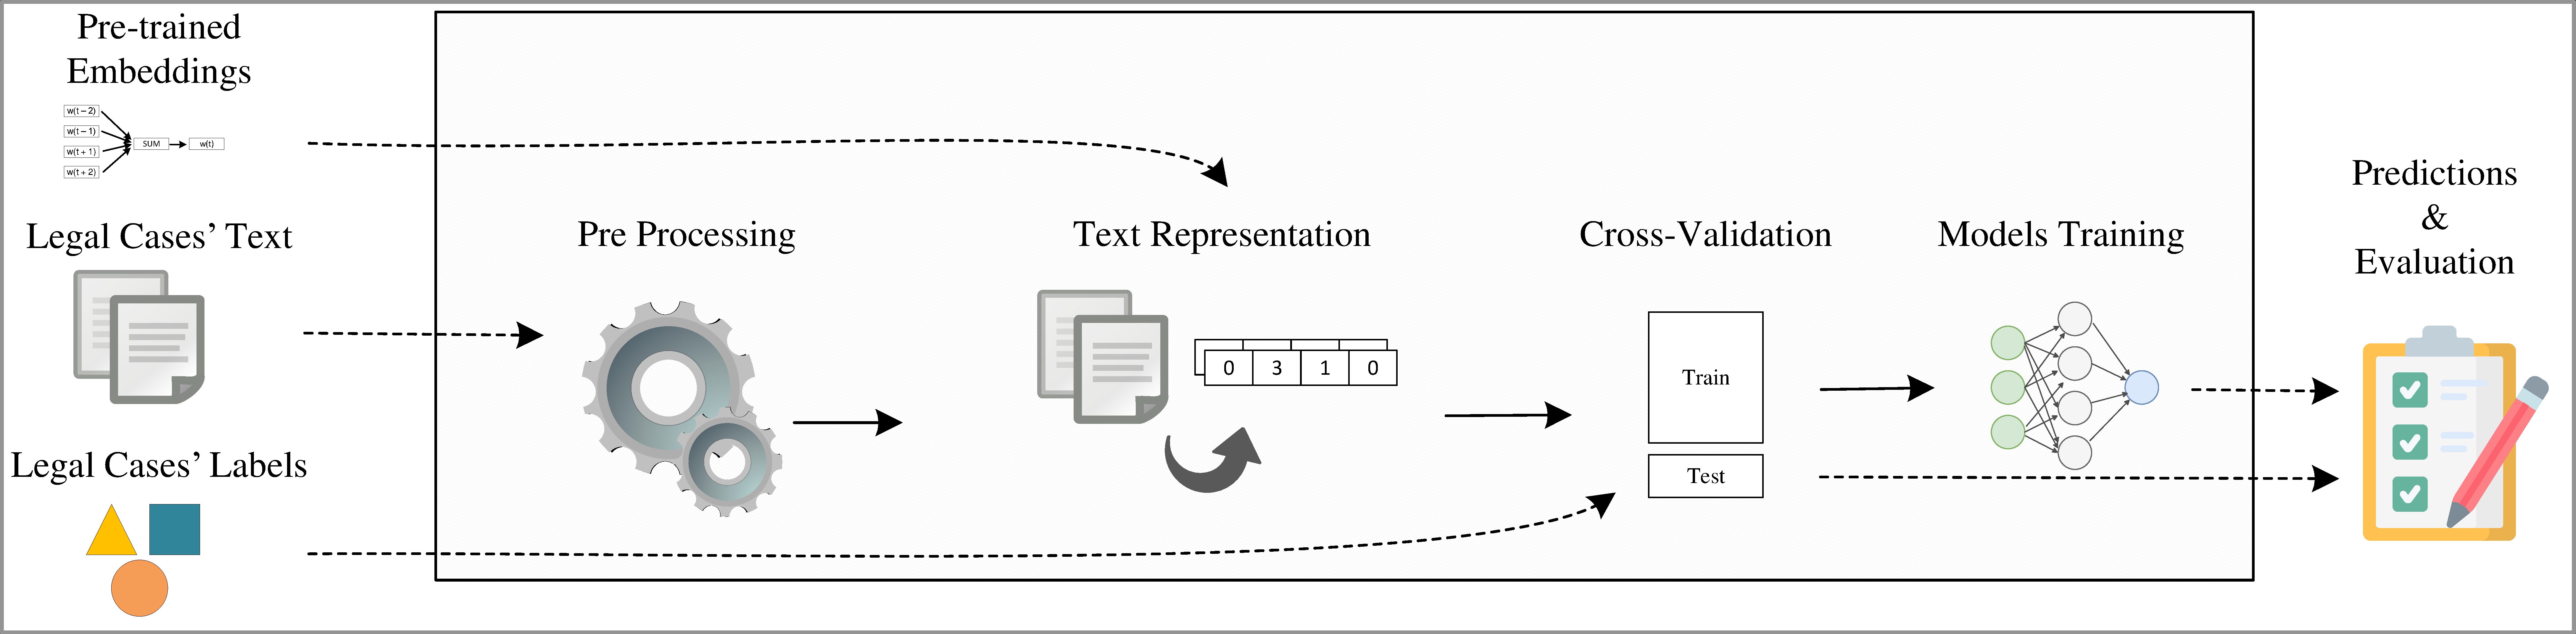
\includegraphics[width=\textwidth]{images/chapters/cap4_proposed_pipeline_dl.pdf}
\end{figure}

Such steps in the pipeline are similar to those in Figure~\ref{fig:cap4_pipeline_superv_ml}, however there are distinct settings. 
Thus, the pipeline receives three types of input: the legal judgments' text, their labels and the pre-trained word embeddings  models. 

Following, the preprocessing step prepares the text to the next steps in the pipeline, however with  different settings from Figure~\ref{fig:cap4_pipeline_superv_ml}. There is the transformation, tokenization using regular expression (\textbackslash w+), however we did not apply stemming or filtering, following the literature~\cite{Mikolov2013, Pennington2014}. Thus, to reproduce the aspects of the corpus applied to the pre-training of the embeddings, their application in ML tasks may not include those preprocessing techniques.
After preprocessing there is the text representation, where pre-trained embeddings techniques were applied. We selected the pre-trained embeddings based on best results in Section~\ref{sec:text_representation}. That is, the word embeddings pre-trained using the corpus related to air transport only. In the referred section, only the GloVe technique was applied and tested due to time limits. However, we later trained other word embeddings in the same corpora to apply in the classification experiments, using the default parameters from Gensim~\cite{Radim2010}.

The next step, cross-validation,  follows the setup from the Classical ML experiments, i.e., the number of folds set to ten. 

Later, there is the models training step, involving three \gls{DL} techniques: \gls{CNN}, \gls{LSTM} and Bi-LSTM with Self Attention. The \gls{CNN} used has the same hyperparemeters  from Section~\ref{sec:text_representation}. 

The \gls{LSTM} architecture, as shown in Figure~\ref{fig:cap4_lstm_model}, receives as input the embeddings, which can be fine-tuned during the training process. Such a setting is enabled in this architecture. The embeddings pass to a Spatial Dropout layer, a regularization method to avoid overfitting on recurrent networks, especially when embeddings can be fine-tuned~\cite{Gal2016}. Then, there is the \gls{LSTM} layer with $100$ units with a dropout and a recurrent dropout of $0.2$. Finally, the output layer corresponds to a Dense Layer with four neurons having sigmoid as activation function.

\begin{figure}[htb]
    \centering
    \caption{LSTM architecture for text classification}
    \label{fig:cap4_lstm_model}
    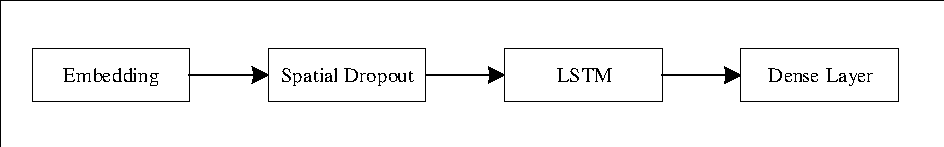
\includegraphics[width=\textwidth]{images/chapters/cap4_lstm_model.pdf}
\end{figure}

% TODO: Definir no C2, LSTM, CNN, Bi-LSTM e Self Attention
The architecture for Bi-LSTM with Self Attention is shown in Figure~\ref{fig:cap4_bilstm_attention_model}. It starts with the Embedding layer followed by Spatial Dropout, both with the same settings from previous \gls{LSTM} model. The Bi-LSTM layer follows, containing 100 units. Then, there is the Many to One Attention step composed of  the Self-Attention, the Concatenation with last Bi-LSTM Hidden State and the Attention Vector. Finally, there is the Dense Layer as the output layer with four neurons with sigmoid activation function.

\begin{figure}[htb]
    \centering
    \caption{Bi-LSTM with Self-Attention architecture for text classification}
    \label{fig:cap4_bilstm_attention_model}
    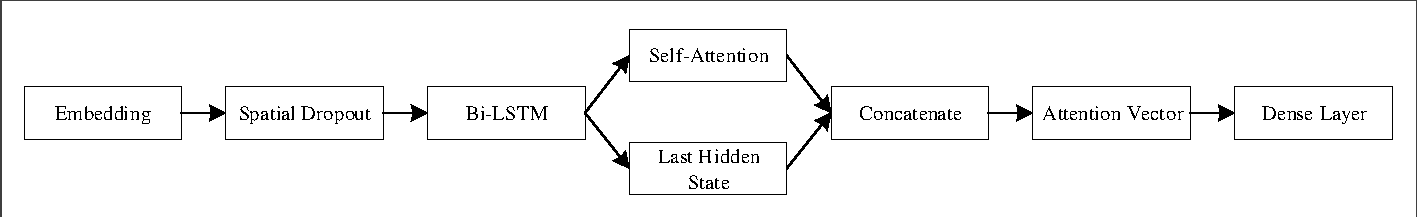
\includegraphics[width=\textwidth]{images/chapters/cap4_bi-lstm_self_attention_model.pdf}
\end{figure}

% Adam with default parameters from Keras.

To run the \gls{DL} experiments based on the architecture from Figure~\ref{fig:pipeline_dl}, distinct setups have been made considering the three \gls{DL} techniques, the two datasets, and the five embeddings models. %Thus, there were thirty combinations of inputs in the experiments.


\subsection{Results and Discussion}


The results obtained after applying the sets of input to the pipelines from Figure~\ref{fig:cap4_pipeline_superv_ml} and~\ref{fig:pipeline_dl} are presented in the following paragraphs.
%
Table~\ref{tab:cap4_class_with_result} details the accuracy obtained by the techniques and representations on each label using the full judgments' text.

% Please add the following required packages to your document preamble:
% \usepackage{booktabs}
% \caption{Acurácia da classificação com o dispositivo das sentenças}
\begin{table}[htb]
\centering
\caption{Classification accuracy for the dataset with judgments' result}
\label{tab:cap4_class_with_result}
\footnotesize
\begin{tabular}{@{}cccrrrrr@{}}
\toprule
\textbf{Technique}&\multicolumn{1}{c}{\textbf{\begin{tabular}[c]{@{}c@{}}Type of\\\gls{ML}\\technique\end{tabular}}} & \textbf{Representation} & \multicolumn{1}{c}{\textbf{\begin{tabular}[c]{@{}c@{}}Well\\ founded\end{tabular}}} & \multicolumn{1}{c}{\textbf{\begin{tabular}[c]{@{}c@{}}Partly\\ founded\end{tabular}}} & \multicolumn{1}{c}{\textbf{\begin{tabular}[c]{@{}c@{}}Not\\ founded\end{tabular}}} & \multicolumn{1}{c}{\textbf{\begin{tabular}[c]{@{}c@{}}Dismissed\\ without\\ prejudice\end{tabular}}} & \multicolumn{1}{c}{\textbf{\begin{tabular}[c]{@{}c@{}}Total\\Acc\end{tabular}}} \\ \midrule
\textbf{\gls{kNN}} & Classical & BOW TF & 75,9\% & 71,9\% & 93,5\% & 95,7\% & 75,8\% \\
\textbf{\gls{LR}} & Classical  & BOW TF & 87,1\% & 86,2\% & 97,6\% & 97,9\% & 87,8\% \\
\textbf{\gls{NB}} & Classical  & BOW TF & 75,2\% & 47,3\% & 91,4\% & 19,6\% & 60,3\% \\
\textbf{\gls{NN}} & Classical  & BOW TF & 85,9\% & 84,9\% & 97,5\% & 97,9\% & 86,7\% \\
\textbf{\gls{RF}} & Classical  & BOW TF & 82,6\% & 82,6\% & 96,1\% & 97,9\% & 84,2\% \\
\textbf{\gls{SVM}} & Classical  & BOW TF & 34,3\% & 45,5\% & 89,6\% & 98,5\% & 47,3\% \\
\textbf{Bi-LSTM-SA} & \gls{DL}& FT CBOW & 81,1\% & 80,4\% & 96,6\% & 98,2\% & 78,1\% \\
\textbf{Bi-LSTM-SA} & \gls{DL} & FT \gls{SG} & 81,1\% & 80,2\% & 97,3\% & 98,5\% & 78,6\% \\
\textbf{Bi-LSTM-SA}  & \gls{DL} & GloVe & 83,1\% & 82,6\% & 96,9\% & 98,2\% & 80,4\% \\
\textbf{Bi-LSTM-SA} & \gls{DL}  & W2V CBOW & 81,3\% & 80,1\% & 97,5\% & 98,4\% & 78,6\% \\
\textbf{Bi-LSTM-SA}  & \gls{DL} & W2V \gls{SG} & 80,8\% & 79,6\% & 97,5\% & 98,4\% & 78,2\% \\
\textbf{\gls{CNN}} & \gls{DL}  & FT CBOW & 48,3\% & 48,9\% & 90,2\% & 98,5\% & 42,9\% \\
\textbf{\gls{CNN}} & \gls{DL}  & FT \gls{SG} & 94,0\% & 94,8\% & 96,9\% & 98,5\% & 92,1\% \\
\textbf{\gls{CNN}}  & \gls{DL} & GloVe & \textbf{97,2\%} & \textbf{97,5\%} & \textbf{98,1\%} & 98,4\% & \textbf{95,5\%} \\
\textbf{\gls{CNN}}  & \gls{DL} & W2V CBOW & 73,0\% & 68,7\% & 90,6\% & 98,5\% & 65,4\% \\
\textbf{\gls{CNN}} & \gls{DL}  & W2V \gls{SG} & 96,0\% & 96,9\% & 97,6\% & 98,5\% & 94,5\% \\
\textbf{\gls{LSTM}} & \gls{DL}  & FT CBOW & 78,2\% & 74,6\% & 90,5\% & 98,5\% & 70,9\% \\
\textbf{\gls{LSTM}}  & \gls{DL} & FT \gls{SG} & 80,2\% & 76,4\% & 92,9\% & 98,5\% & 74,0\% \\
\textbf{\gls{LSTM}} & \gls{DL}  & GloVe & 80,7\% & 78,6\% & 96,1\% & 98,5\% & 77,0\% \\
\textbf{\gls{LSTM}}  & \gls{DL} & W2V CBOW & 77,4\% & 73,8\% & 89,6\% & 98,5\% & 69,7\% \\
\textbf{\gls{LSTM}} & \gls{DL}  & W2V \gls{SG} & 78,6\% & 73,7\% & 91,8\% & 98,5\% & 71,3\% \\ \bottomrule
\end{tabular}

%\fonte{\textcite{Sabo2019}.}
\end{table}


% O que escrever aqui?
% Primeiro dizer o óbvio: qual a ordem da melhor pra pior?
% CNNs..., LR e tudo mais
% CNN foi muito bem, soube detectar bem quais palavras tem alguma relação com o resultado.
% E as demais técnicas, o que mudou?
% Diferença entre os resultados dos embeddings.
% Em relação às classes? continua igual?
% WF: CNN Glove, W2V SG, FT SG, 
% PF: idme
% NF:
% DWJ: 
% TOAL:
% Pq? 
% - Possíveis causas para bom resultado:
%       Facilidade em relacionar o texto descrito com o resultado, mas não uma capacidade de "raciocinar" 


From Table~\ref{tab:cap4_class_with_result}, one can notice that most techniques achieved accuracies superior to 70\%, indicating good results on the classification of legal judgments from \gls{JEC}. In terms of techniques' performances, the CNN with GloVe embeddings achieved the best accuracies for the  \emph{Well Founded}, \emph{Partially Founded},  \emph{Not founded} labels and for the total accuracy. The \gls{CNN} also achieve good results when combined with the Word2Vec \gls{SG} and FastText \gls{SG}. Besides \gls{CNN}, the next techniques with best performances are Classical \gls{ML} techniques, that is, \gls{LR}, \gls{NN} and \gls{RF}. 

In terms of worst results, the \gls{CNN} with FastText \gls{CBOW} embeddings achieved the smallest total accuracy, followed by \gls{SVM}, Naïve Bayes and \gls{CNN} with Word2Vec CBOW. Regarding labels, on the other hand,  \gls{SVM} achieved the worst results for the  \emph{Well Founded}, \emph{Partially Founded},  \emph{Not founded}, and the Naïve Bayes for the \emph{Dismissed without Prejudice} label.



The second part of experiments on Classical \gls{ML} and \gls{DL} related to the classification of legal judgments from \gls{JEC} without the judgments' result. Table~\ref{tab:cap4_class_without_result} contains the accuracy achieved by each technique and representation for the four labels and total accuracy using the text of the judgments without result. 


\begin{table}[htb]
\centering
\caption{Classification accuracy for the dataset without judgments' result}
\label{tab:cap4_class_without_result}
\footnotesize
\begin{tabular}{@{}cccrrrrr@{}}
\toprule
\textbf{Technique} &\multicolumn{1}{c}{\textbf{\begin{tabular}[c]{@{}c@{}}Type of\\\gls{ML}\\technique\end{tabular}}} & \textbf{Representation} & \multicolumn{1}{c}{\textbf{\begin{tabular}[c]{@{}c@{}}Well\\ Founded\end{tabular}}} & \multicolumn{1}{c}{\textbf{\begin{tabular}[c]{@{}c@{}}Partly\\ founded\end{tabular}}} & \multicolumn{1}{c}{\textbf{\begin{tabular}[c]{@{}c@{}}Not\\ founded\end{tabular}}} & \multicolumn{1}{c}{\textbf{\begin{tabular}[c]{@{}c@{}}Dismissed\\ without\\ prejudice\end{tabular}}} & \multicolumn{1}{c}{\textbf{\begin{tabular}[c]{@{}c@{}}Total\\Acc\end{tabular}}} \\ \midrule
\textbf{kNN} & Classical & BOW TF & 75,2\% & 72,1\% & 90,9\% & 93,2\% & 75,4\% \\
\textbf{LR} & Classical  & BOW TF & 80,7\% & 79,2\% & 94,9\% & 97,9\% & 81,6\% \\
\textbf{NB} & Classical  & BOW TF & 74,3\% & 46,5\% & 90,2\% & 18,1\% & 59,5\% \\
\textbf{NN} & Classical  & BOW TF & 81,0\% & 79,0\% &\textbf{ 95,1\%} & 97,9\% & 81,6\% \\
\textbf{RF}  & Classical & BOW TF & \textbf{82,2\%} & \textbf{79,9\%} & 92,7\% & 97,9\% & \textbf{82,2\%} \\
\textbf{\gls{SVM}} & Classical  & BOW TF & 33,4\% & 45,0\% & 89,6\% & 98,5\% & 46,7\% \\
\textbf{Bi-LSTM-SA} & \gls{DL} & FT CBOW & 79,5\% & 77,1\% & 94,3\% & 98,5\% & 74,7\% \\
\textbf{Bi-LSTM-SA}  & \gls{DL} & FT \gls{SG} & 78,5\% & 75,8\% & 94,6\% & 98,5\% & 73,7\% \\
\textbf{Bi-LSTM-SA}  & \gls{DL} & GloVe & 79,9\% & 77,3\% & 94,8\% & 98,4\% & 75,2\% \\
\textbf{Bi-LSTM-SA} & \gls{DL}  & W2V CBOW & 79,5\% & 76,7\% & 93,9\% & 98,5\% & 74,3\% \\
\textbf{Bi-LSTM-SA}  & \gls{DL} & W2V \gls{SG} & 80,4\% & 77,4\% & 93,8\% & 98,5\% & 75,0\% \\
\textbf{CNN}  & \gls{DL} & FT CBOW & 50,5\% & 51,7\% & 89,9\% & 98,5\% & 45,3\% \\
\textbf{CNN}  & \gls{DL} & FT \gls{SG} & 80,8\% & 78,0\% & 93,0\% & 98,5\% & 75,2\% \\
\textbf{CNN} & \gls{DL}  & GloVe & 80,4\% & 77,3\% & 93,0\% & 98,5\% & 74,6\% \\
\textbf{CNN}  & \gls{DL} & W2V CBOW & 66,6\% & 58,7\% & 90,0\% & 98,5\% & 56,9\% \\
\textbf{CNN} & \gls{DL}  & W2V \gls{SG} & 81,7\% & 79,5\% & 93,3\% & 98,5\% & 76,5\% \\
\textbf{LSTM}  & \gls{DL} & FT CBOW & 79,8\% & 71,3\% & 88,6\% & 98,5\% & 69,1\% \\
\textbf{LSTM}  & \gls{DL} & FT \gls{SG} & 77,5\% & 69,1\% & 88,1\% & 98,5\% & 66,6\% \\
\textbf{LSTM} & \gls{DL}  & GloVe & 81,1\% & 74,7\% & 91,2\% & 98,5\% & 72,8\% \\
\textbf{LSTM}  & \gls{DL} & W2V CBOW & 80,8\% & 73,7\% & 87,8\% & 98,5\% & 70,4\% \\
\textbf{LSTM} & \gls{DL}  & W2V \gls{SG} & 79,2\% & 72,4\% & 88,4\% & 98,5\% & 69,2\% \\ \bottomrule
\end{tabular}

%\fonte{\textcite{Sabo2019}.}
\end{table}

The results show the sequence of best techniques has changed, as the Classical ML techniques \gls{RF}, \gls{LR} and \gls{NN} achieved the best total accuracies followed by the \gls{CNN} with Word2Vec \gls{SG}. In terms of labels, the RF performed better for the \emph{Well founded} and  \emph{Partially founded}, while \gls{NN} performed better with \emph{Not founded}. For the label \textit{Dismissed without prejudice}, several classes achieved good results, although it has the smallest sample. On the other hand, similar to the results from Table~\ref{tab:cap4_class_with_result}, the techniques with worse performance were the \gls{CNN} with FastText CBOW followed by \gls{SVM} and \gls{CNN} with Word2Vec CBOW.


% Results para colocar aqui
% 
% A CNN ele se saiu muito bem com resultado e não tão bem sem  o resultado o que mostra que ela conseguiu relacionar muito bem o trecho da sentença com o label do doc, isto é. A CNN identificou a sentença como uma parte muito importante do documento.
% Além disso, percebeu-se a importância da técnicna de representação, uma que vez que simplesmente alterando a representação utilizada na CNN fez que com ela tivesse tanto resultados muito bons quanto muito ruins.
% Deixar claro que o caso prático seria usar o texto sem a sentença final, apenas contentdo o resumo do caso e as leis aplicáveis. Portanto que num caso real no JEC, as técnicas de Classical ML seriam mais adequadas para a classificação.


In general, it is inferred that the accuracy in the experiment with the removal of the judgments' result (part of the text indicating the label to which it belongs) suffered a minimal reduction for the Classical ML techniques as well as LSTM and Bi-LSTM-SA, which demonstrates that the classifiers were able to maintain their performance with the text in which the facts narrated by the parties to the process are reported and the legal grounds applicable to the case. 
However, for the CNN there was a significant decay in performance when removing the cases' result. And, such  decay in performance may show the technique inferred that the text from the result part  had significant information for the classification of the legal cases.
However, the removal of such part made it harder for the CNN to infer the judgment's label based on remaining two parts of the text. 

Another observation for the CNN is the impact of the representations in the performance of the technique, as changing the representation used in the pipeline was enough to reduce the accuracy by more than 30\% when comparing to the best CNN results. However, for the other two DL techniques, LSTM and Bi-LSTM with Self Attention, the differences in performance while shifting representations were significantly smaller.

% Esse fica como último parágrafo.
Finally, a good performance when classifying the judgments without results becomes a prerequisite for carrying out experiments with texts from legal proceedings in which there is still no sentence, that is, in which the judge has not yet decided the result. In this case, the best choice may be the use of Classical ML techniques, such as LR and RF, as they perform better on the classification task than DL techniques and due to the fact those models are less complex and require less examples to train.
The \gls{DL} techniques, especially CNN with GloVe may be useful inside JEC when the objective is to organize existing judgments by categories such as their labels or matters, for example. 

This conclusions are limited to our small dataset from \gls{JEC}. Thus, if we had a larger dataset with more training examples, the \gls{DL} would possibly achieve better results.


% Place this in Conclusions Chapter
% \subsection{Conclusions from the section}

% The experiments from this section dealt with initial experiments carried out in the sentences of the JEC/UFSC, indicating only four possible classes to which the texts belong. In general, it was possible to obtain an overview of how the several ML techniques behave in the face of legal texts (specific on Consumer Law and failure in air transport service), evaluating which classification models reached higher and lower accuracy.

%As future works, the aim is to improve the text representation of the bag of words for a more robust representation, such as Word Embeddings, capable of numerically associating contexts and semantics to words. In addition, we intend to build a new structure for sentence prediction, composed of cascading classifiers, using attributes extracted from texts through clustering. Thus, it is possible to make intermediate classifications that will serve as a basis for a final classification. 





